% !TEX program = xelatex
\documentclass[aspectratio=1610,8pt]{beamer}
\usepackage[utf8]{inputenc}
\usepackage[T1]{fontenc}
\usepackage{lmodern}
\usepackage{caption,subcaption}
\usepackage{multirow}
\usepackage{multicol}
\usepackage{comment}
\usepackage{csquotes}
\usepackage[maxbibnames=99]{biblatex}
\usepackage[makeroom]{cancel}
\usepackage{threeparttable}
\usepackage{tikzsymbols}
\usepackage{textcomp}
\usepackage{parskip}
\usepackage{pgf}
\usepackage{color,soul}
\usepackage[listings,theorems]{tcolorbox}
\tcbuselibrary{skins}
\usepackage{hyperref}
\usepackage{xcolor,soul}
\usepackage{empheq}
\usepackage{enumerate}
\usepackage{collcell}
\usepackage{booktabs}
\usepackage{etoolbox}
\usepackage{xcoffins}
\usepackage{pgfpages}
\usepackage{stackengine,tikz}
\usepackage{transparent}
\usepackage{eqnarray,amsmath}
\usepackage{amsfonts}
\usepackage{amssymb}
\usepackage{mathtools}
\usepackage{expl3}
\usepackage[vietnamese]{babel}

\usetheme{Madrid}

% Modern color scheme
\definecolor{primaryblue}{RGB}{0,90,156}
\definecolor{accentblue}{RGB}{100,143,255}
\definecolor{textgray}{RGB}{66,66,66}
\definecolor{lightgray}{RGB}{245,245,245}
\definecolor{cvut_navy}{HTML}{0065BD}
\definecolor{cvut_blue}{HTML}{6AADE4}
\definecolor{lightgreen}{HTML}{90EE90}
\definecolor{darksalmon}{rgb}{0.91, 0.59, 0.48}
\definecolor{darkred}{RGB}{180,0,0}
\definecolor{darkgreen}{RGB}{0,120,0}

% Block colors
\AtBeginDocument{
  \setbeamercolor{block title}{use=structure,fg=white,bg=primaryblue}
  \setbeamercolor{block body}{use=structure,fg=black,bg=white}
  \setbeamercolor{block title alerted}{use=alerted text,fg=white,bg=red!75}
  \setbeamercolor{block body alerted}{fg=black,bg=white}
  \setbeamercolor{block title example}{use=example text,fg=white,bg=accentblue}
  \setbeamercolor{block body example}{fg=black,bg=lightgray}
}

% Other color configurations
\sethlcolor{lightblue}
\setbeamercolor{section in toc}{fg=black,bg=yellow} 
\setbeamercolor{alerted text}{fg=cvut_blue}
\setbeamercolor{palette primary}{bg=primaryblue,fg=white}
\setbeamercolor{palette secondary}{bg=primaryblue,fg=white}
\setbeamercolor{palette tertiary}{parent=palette primary}
\setbeamercolor{palette quaternary}{fg=primaryblue,bg=lightgray}
\setbeamercolor{sidebar}{fg=primaryblue,bg=white}
\setbeamercolor{titlelike}{parent=palette primary}
\setbeamercolor{frametitle}{bg=white,fg=primaryblue}
\setbeamercolor{B}{bg=accentblue!20,fg=textgray}
\setbeamercolor{itemize item}{fg=primaryblue}

\hypersetup{
    urlcolor=blue, 
    linkcolor=darksalmon, 
    citecolor=blue,
    colorlinks=true
}

\addbibresource{references.bib}

\renewcommand<>{\hl}[1]{\only#2{\beameroriginal{\hl}}{#1}}
\newcommand{\boxedeq}[2]{\begin{empheq}[box={\fboxsep=6pt\fbox}]{align}\label{#1}#2\end{empheq}}

\setbeamertemplate{caption}[numbered]
\useoutertheme{infolines}
\setbeamertemplate{page number in head/foot}[framenumber]
\setbeamertemplate{section in toc}[default]
\setbeamertemplate{itemize item}[circle]
\setbeamertemplate{subsection in toc}[subsections numbered]
\setbeamertemplate{navigation symbols}{} 
\setbeamertemplate{caption}{\raggedright\insertcaption\par}
\usefonttheme{professionalfonts}

\setbeamertemplate{headline}{%
\begin{beamercolorbox}[colsep=1.5pt]{upper separation line head}
\end{beamercolorbox}
\begin{beamercolorbox}{section in head/foot}
    \vskip2pt\insertsectionnavigationhorizontal{\paperwidth}{}{\hskip0pt plus1filll}\vskip2pt
\end{beamercolorbox}%
\begin{beamercolorbox}[colsep=1.5pt]{lower separation line head}
\end{beamercolorbox}
}

\setbeamercovered{dynamic}

%====================================================
%========== TITLE INFORMATION =======================
%====================================================
\institute[HCMUT]{
\vspace{-1cm}
\begin{center}
    \includegraphics[height=1.25cm]{Beamer/hcmut.png}
\end{center}
\vspace{0.1cm}
\Large{\scriptsize{\textbf{\color{black}BÁO CÁO THỰC TẬP 1}}} \\ \textbf{BÁO CÁO LẦN 2}\\
% \textbf{Visual Grounding for Hallucination Reduction}
\\[0.5cm]
\scriptsize{
\begin{table}[h]
\centering
    \begin{tabular}{ll}
        \color{blue}Học viên thực hiện: & \textbf{Võ Phạm Tuấn Dũng - 2570015} \\
    \end{tabular}
\end{table}
}
}

\title[]{\normalsize\textsf{TRƯỜNG ĐẠI HỌC BÁCH KHOA - ĐHQG TP.HCM\\KHOA KHOA HỌC VÀ KỸ THUẬT MÁY TÍNH}}

\date[Oct 2025]{ \\ \scriptsize{TP.HCM, tháng 1 năm 2025}}

%====================================================
\AtBeginSection[]{
  \begin{frame}<beamer>
    \frametitle{Nội dung}
    \tableofcontents[currentsection,currentsubsection]
  \end{frame}
}

\begin{document}

\begin{frame}[plain]{}
	\titlepage
\end{frame}

\begin{frame}[plain]{\textbf{Nội dung báo cáo}}
\tableofcontents[]
\end{frame}










%====================================================
\section{Giới thiệu CoRGI}

\begin{frame}{CoRGI là gì?}
\begin{itemize}
    \item \textbf{CoRGI (Chain of Reasoning with Grounded Insights)} nâng cao độ tin cậy suy luận của VLM bằng cách hậu kiểm từng bước chain-of-thought với chứng cứ thị giác.
    \item Khắc phục hiện tượng \textit{single-look bias}: mô hình mô tả lưu loát nhưng trôi khỏi nội dung ảnh dẫn tới hallucination.
    \item Pipeline trong Gradio demo theo dõi đồng bộ reasoning, evidence và key evidence để người dùng hiểu rõ vì sao mô hình trả lời.
\end{itemize}
\end{frame}

\begin{frame}{Vấn đề và cách tiếp cận}
\begin{itemize}
    \item CoRGI cho phép VLM sinh đầy đủ chuỗi suy luận, sau đó mới tiến hành xác minh hậu kiểm thay vì buộc mô hình quan sát nhiều lần.
    \item Không cần iterative grounding hay huấn luyện lại đắt đỏ, tương thích với các VLM có sẵn.
    \item Kết hợp \textbf{Qwen3-VL-2B-Instruct} (Stage 1 \& 4) và \textbf{Florence-2-large-ft} (Stage 2 \& 3) để vừa suy luận tốt vừa grounding chính xác.
    \item Đầu ra tiêu chuẩn: câu trả lời ngắn gọn, giải thích 2--3 câu và key evidence (tọa độ bbox) cho người dùng kiểm chứng.
\end{itemize}
\end{frame}

%====================================================
\section{Kiến trúc Pipeline}

\begin{frame}{Sơ lược kiến trúc CoRGI}
\begin{columns}[T]
\column{0.56\textwidth}
\begin{figure}
    \centering
    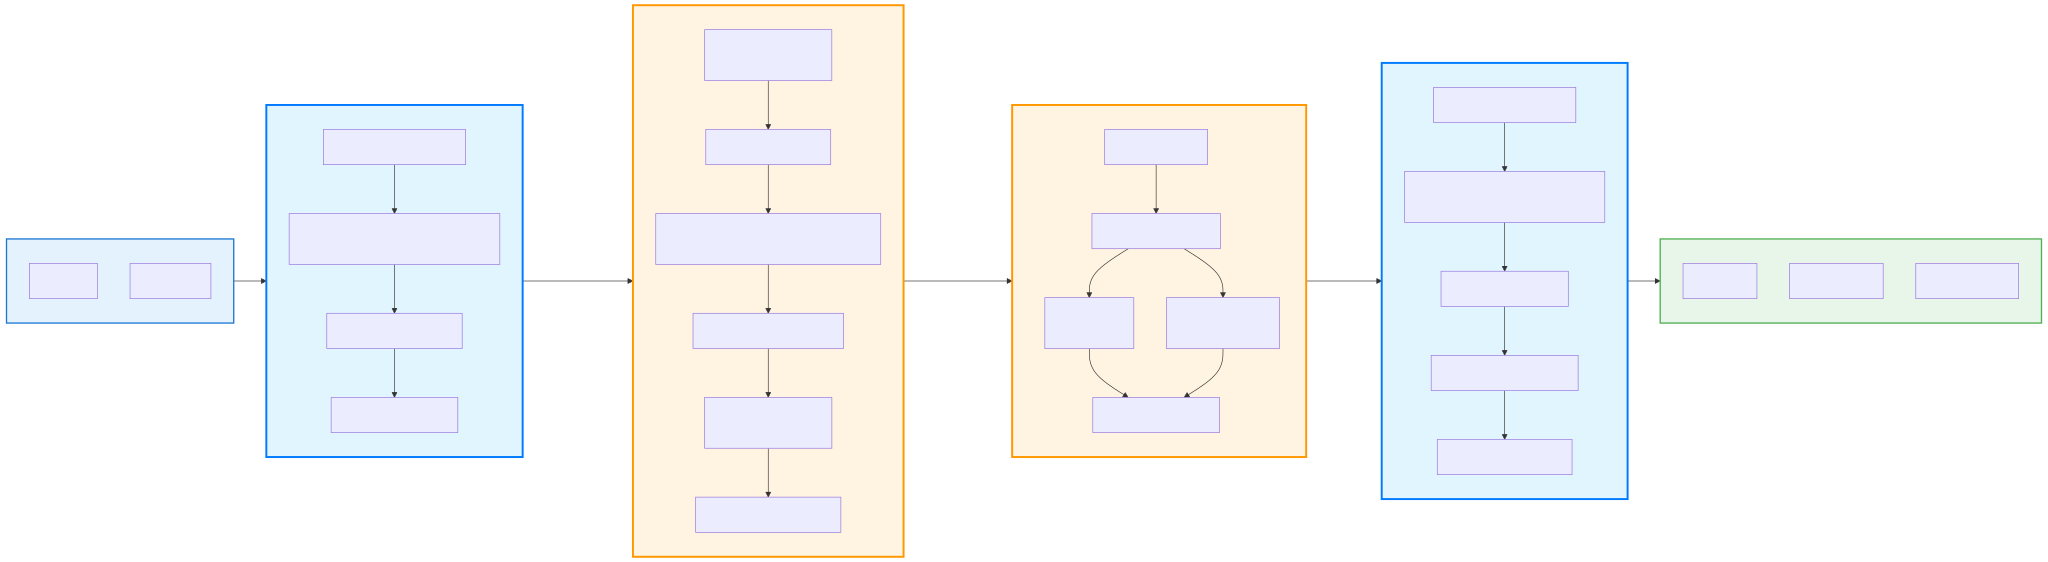
\includegraphics[width=\linewidth]{pipeline_architecture.png}
    \caption{Kiến trúc 4 stage trong demo}
\end{figure}
\column{0.44\textwidth}
\begin{itemize}
    \item \textbf{Stage 1}: Qwen3-VL sinh chain-of-thought + noun phrase cho từng bước.
    \item \textbf{Stage 2}: Florence-2 grounding các noun phrase thành bbox, áp dụng IoU-based NMS.
    \item \textbf{Stage 3}: Florence-2 chạy OCR \& caption song song trên từng vùng.
    \item \textbf{Stage 4}: Qwen3-VL tổng hợp answer, explanation và key evidence từ toàn bộ chứng cứ.
\end{itemize}
\end{columns}
\end{frame}

\begin{frame}{Luồng xử lý từng bước}
\small
\begin{enumerate}
    \item \textbf{Input}: người dùng tải ảnh và câu hỏi.
    \item \textbf{Reasoning}: Qwen3-VL tạo chain-of-thought + JSON bước với cờ ``needs\_vision'' và ``need\_ocr''.
    \item \textbf{Grounding}: Florence-2 trích tọa độ vùng liên quan cho từng bước cần nhìn ảnh.
    \item \textbf{NMS}: loại trừ bbox chồng lấn để tránh trùng lặp bằng chứng.
    \item \textbf{Evidence}: từng vùng được crop một lần rồi chạy OCR \& caption song song.
    \item \textbf{Synthesis}: Qwen3-VL kết hợp câu hỏi, bước suy luận và mô tả vùng để suy ra câu trả lời + giải thích.
    \item \textbf{Output}: trả về answer, giải thích và tối đa 1 key evidence (bbox + mô tả).
\end{enumerate}
\end{frame}

%====================================================
\section{Cấu hình mô hình}

\begin{frame}{Bảng cấu hình mô hình}
\begin{table}[h]
\scriptsize\centering
\begin{tabular}{p{0.18\textwidth}p{0.2\textwidth}p{0.22\textwidth}p{0.32\textwidth}}
\toprule
Stage & Model & Mục đích & Tính năng chính \\
\midrule
Stage 1: Reasoning & Qwen3-VL-2B-Instruct & Sinh chuỗi suy luận có cấu trúc & Chain-of-Thought 2--4 câu\\JSON steps \& noun phrase\\Cờ needs\_vision/need\_ocr \\
Stage 2: Grounding & Florence-2-large-ft & Tìm bounding box cho từng noun phrase & Phrase grounding\\Loại bỏ trùng qua IoU\\Thích ứng cả implicit lẫn explicit tham chiếu \\
Stage 3: Evidence & Florence-2-large-ft & Mô tả nội dung vùng (OCR + Caption) & Crop một lần cho 2 tác vụ\\Chạy song song\\Mô tả chi tiết nội dung hình/ chữ \\
Stage 4: Synthesis & Qwen3-VL-2B-Instruct & Tổng hợp answer + key evidence & Ràng buộc JSON rõ ràng\\Ưu tiên evidence quan trọng\\Sinh giải thích ngắn gọn \\
\bottomrule
\end{tabular}
\end{table}
\end{frame}

%====================================================
\section{Khác biệt so với paper gốc}

\begin{frame}{Điều chỉnh chính}
\begin{columns}[T]
\column{0.48\textwidth}
\textbf{Lựa chọn mô hình}
\begin{itemize}
    \item Stage 1 \& 4 dùng Qwen3-VL-2B-Instruct thay vì Qwen-2.5VL, LLaVA1.6 hay Gemma3-12B trong paper gốc.
    \item Stage 2 \& 3 dùng Florence-2-large-ft thay Grounding DINO để tận dụng OCR/caption tích hợp.
\end{itemize}
\column{0.48\textwidth}
\textbf{Cấu trúc pipeline}
\begin{itemize}
    \item Chia rõ 4 stage: ROI extraction và evidence description tách biệt để dễ tối ưu.
    \item Bỏ classifier riêng: cờ ``needs\_vision'' được sinh trực tiếp từ reasoning output.
\end{itemize}
\end{columns}
\end{frame}

\begin{frame}{Tối ưu hoá và lợi ích triển khai}
\begin{columns}[T]
\column{0.48\textwidth}
\textbf{Optimizations \& Enhancements}
\begin{itemize}
    \item IoU-based NMS giảm vùng trùng lặp, tập trung vào evidence hữu ích.
    \item Parallel OCR + captioning trên mỗi crop để rút ngắn thời gian.
    \item Không cần text reranker riêng, evidence được dùng trực tiếp.
    \item Kiến trúc mô-đun: dễ thay thế model qua file YAML.
\end{itemize}
\column{0.48\textwidth}
\textbf{Implementation Benefits}
\begin{itemize}
    \item Lightweight: không huấn luyện thêm classifier phức tạp.
    \item Efficient: tối ưu cho Hugging Face Spaces với quản lý GPU context và batch captioning.
    \item Flexible: cấu hình YAML giúp chỉnh model/siêu tham số nhanh.
    \item Production-ready: xử lý lỗi toàn diện, chuẩn hoá hệ tọa độ, logging rõ ràng.
\end{itemize}
\end{columns}
\end{frame}

%====================================================
\section{Prompt Templates}

\begin{frame}[fragile]{Stage 1: Chain-of-Thought reasoning}
\begin{itemize}
    \item \textbf{Model}: Qwen3-VL-2B-Instruct sinh chain-of-thought 2--4 câu và JSON step (tối đa 3 bước).
    \item Statement bắt buộc là noun phrase, reason <=5 từ, xác định rõ ``need\_ocr''.
    \item Đầu ra phải tuân thủ định dạng JSON cố định để chuyển xuống Stage 2.
\end{itemize}

{\scriptsize
\begin{verbatim}
You are a careful multimodal reasoner analyzing an image to answer a question.

Question: What is the color of the watch?

# Steps to verify:
{
  "steps": [
    {
      "index": 1,
      "statement": "specific noun phrase identifying target object/region",
      "needs_vision": true,
      "need_ocr": false,
      "reason": "brief 3-5 word reason"
    }
  ]
}
\end{verbatim}}
\end{frame}

\begin{frame}[fragile]{Stage 2: ROI Extraction (Grounding)}
\begin{itemize}
    \item \textbf{Model}: Florence-2-large-ft với tác vụ <CAPTION\_TO\_PHRASE\_GROUNDING>, có thể dùng prompt Qwen khi cần.
    \item Trả về tối đa 3 bbox theo tọa độ [0, 999] cho mỗi bước cần nhìn ảnh.
    \item Phản hồi bắt buộc là JSON thuần (evidences, bbox, description, confidence).
\end{itemize}

{\scriptsize
\begin{verbatim}
You are validating the following reasoning step:
the watch on the woman's wrist

REQUIRED JSON FORMAT (bboxes in [0-999] coordinate range):
{
  "evidences": [
    {
      "step": 1,
      "bbox": [x1, y1, x2, y2],
      "description": "visual description",
      "confidence": 0.95
    }
  ]
}
\end{verbatim}}
\end{frame}

\begin{frame}[fragile]{Stage 3: Evidence Description}
\begin{itemize}
    \item \textbf{Model}: Florence-2-large-ft chạy hai tác vụ <OCR> và <MORE\_DETAILED\_CAPTION> song song.
    \item Mỗi vùng được crop đúng một lần để dùng chung cho OCR và captioning.
    \item Prompt nhắc lại statement nhằm giữ ngữ cảnh cho mô tả.
\end{itemize}

{\scriptsize
\begin{verbatim}
Describe precisely what is visible in this cropped region in 1-2 sentences.
Focus only on directly observable details.
Avoid speculation.

Context: This region is being examined to verify the statement: "the watch on the woman's wrist"
\end{verbatim}}
\end{frame}

\begin{frame}[fragile]{Stage 4: Answer Synthesis}
\begin{itemize}
    \item \textbf{Model}: Qwen3-VL-2B-Instruct tổng hợp câu hỏi, bước suy luận và evidence.
    \item Ràng buộc quan trọng: tối đa 1 key evidence, trả lời ngắn gọn nhưng có giải thích liên kết evidence.
    \item Đáp án phải theo JSON với thứ tự trường cố định (answer → explanation → key\_evidence).
\end{itemize}

{\scriptsize
\begin{verbatim}
You are finalizing the answer using verified evidence.

Question: What is the color of the watch?

Structured reasoning steps:
1. the watch on the woman's wrist (needs vision: True)

Verified visual evidence:
Step 1: bbox=(539, 571, 568, 612), conf=0.95, desc=A person is wearing a white watch on their wrist.

{
  "answer": "Final answer",
  "explanation": "Brief explanation connecting evidence to answer",
  "key_evidence": [
    {
      "bbox": [x1, y1, x2, y2],
      "description": "What this region shows",
      "reasoning": "Why this supports the answer"
    }
  ]
}
\end{verbatim}}
\end{frame}

%====================================================
\section{Kỹ thuật triển khai}

\begin{frame}{Kỹ thuật triển khai (1/2)}
\begin{block}{1. Non-Maximum Suppression (NMS)}
\begin{itemize}
    \item Mục tiêu: loại bỏ bbox chồng lấn từ Florence-2.
    \item Phương pháp: lọc theo IoU với ngưỡng cấu hình (mặc định 0.5).
    \item Lợi ích: giảm redundancy, tập trung vào vùng quan trọng.
\end{itemize}
\end{block}
\begin{block}{2. Parallel OCR \& Captioning}
\begin{itemize}
    \item Thực thi song song bằng \texttt{ThreadPoolExecutor}, chia sẻ cùng crop ảnh.
    \item Hợp nhất kết quả để có mô tả chi tiết lẫn text.
\end{itemize}
\end{block}
\begin{block}{3. KV Cache Optimization}
\begin{itemize}
    \item \texttt{use\_cache=True} cho Qwen giúp giảm thời gian suy luận đa bước.
    \item Florence-2 bỏ cache do giới hạn transformers hiện tại.
\end{itemize}
\end{block}
\end{frame}

\begin{frame}{Kỹ thuật triển khai (2/2)}
\begin{block}{4. Fast Image Processor}
\begin{itemize}
    \item Ưu tiên \texttt{use\_fast=True} để rút ngắn tiền xử lý, fallback sang bản chậm khi cần.
    \item Áp dụng nhất quán cho mọi model loader.
\end{itemize}
\end{block}
\begin{block}{5. Coordinate System Handling}
\begin{itemize}
    \item Chuẩn hoá tự động giữa tọa độ chuẩn hoá, [0,999] và pixel tuyệt đối.
    \item Utility \texttt{coordinate\_utils.py} dò định dạng rồi chuyển đổi tương thích giữa Qwen và Florence-2.
\end{itemize}
\end{block}
\end{frame}

\end{document}
